\documentclass[aspectratio=169]{beamer}

% Suppress all navigation symbols
\setbeamertemplate{navigation symbols}{}
\setbeamertemplate{headline}{}
\setbeamertemplate{footline}{}
\setbeamertemplate{itemize items}[circle]
\setbeamertemplate{footline}[frame number]

\setbeamercolor{structure}{fg=blue}
\setbeamercolor{normal text}{fg=black, bg=white}
\setbeamerfont{title}{series=\bfseries, size=\Huge}
\setbeamerfont{frametitle}{series=\bfseries, size=\LARGE}

\setbeamertemplate{footline}{
  \begin{tikzpicture}[remember picture,
                      overlay,
                      shift={(current page.south west)}]
    \node [black!50, inner sep=2mm, anchor=south east]
          at (current page.south east)
          {\large \bfseries \insertframenumber};
  \end{tikzpicture}
}

\definecolor{red}{RGB}{220, 50, 47}
\definecolor{green}{RGB}{133, 153, 0}
\definecolor{cyan}{RGB}{42, 161, 152}
\definecolor{blue}{RGB}{38, 139, 210}
\definecolor{yellow}{RGB}{181, 137, 0}

\usepackage{fontspec}
\setsansfont{Overpass}[Scale=MatchLowercase]
\setmonofont{Overpass Mono}[Scale=MatchLowercase]

\usepackage{listings}
\lstset{
  basicstyle=\ttfamily\small,
  commentstyle={\color{black!50}},
  language=Java,
}

\usepackage{pgfplots}

\usepackage{tikz}
\usetikzlibrary{arrows}
\usetikzlibrary{backgrounds}
\usetikzlibrary{calc}
\usetikzlibrary{decorations.pathreplacing}
\usetikzlibrary{fit}
\usetikzlibrary{positioning}
\usetikzlibrary{matrix}
\usetikzlibrary{scopes}
\usetikzlibrary{shapes}
\usetikzlibrary{tikzmark}
\usetikzmarklibrary{listings}

\title{JInline}
\author{Jonathan Eyolfson and Christian Navasca}
\date{2020-02-26}

\setbeamertemplate{title page}
{
  \begin{tikzpicture}[remember picture,
                      overlay,
                      shift={(current page.south west)}]
    \node (title) [inner sep=0, scale=1.2, align=center]
          at (\paperwidth / 2, \paperheight * 2 / 3)
          {\usebeamerfont{title}\usebeamercolor[fg]{title} \inserttitle};
    \node (author) [scale=1.5] at (\paperwidth / 2, \paperheight / 3)
          {\insertauthor};
    \node [anchor=south east, inner sep=2mm] at (\paperwidth, 0)
          {\bfseries \insertdate};
  \end{tikzpicture}
}

\begin{document}

  \begin{frame}[plain]
    \titlepage
  \end{frame}

  \setcounter{framenumber}{0}

  \begin{frame}[fragile]
    \frametitle{Inlining May Enable Library Removal}

    \begin{columns}[t]
      \begin{column}{0.5\textwidth}
        \hspace{3.4em} \structure{Before}
        \begin{lstlisting}[xleftmargin=4em]
public class Application {
  // ...
  public void bar() {
    int x = a.foo();
  }
  // ...
}

public class LibraryA {
  // ...
  public int foo() {
    return /* complex */;
  }
  // ...
}
        \end{lstlisting}
      \end{column}
      \begin{column}{0.5\textwidth}
        \hspace{3.4em} \structure{After}
        \begin{lstlisting}[xleftmargin=4em]
public class Application {
  // ...
  public void bar() {
    int x = /* complex */;
  }
  // ...
}
        \end{lstlisting}
      \end{column}
    \end{columns}
    \begin{tikzpicture}[remember picture,
                        overlay,
                        shift={(current page.south west)}]
      \draw [blue, ->, >=stealth']
        ($(current page.center)+(-4em,-6.8em)$)
        -- node [above left, align=center, blue]
        {\footnotesize Inline \texttt{foo}}
        ($(current page.center)+(4em,0)$);
      \draw [blue, ->, >=stealth']
        ($(current page.center)+(-4em,-6.8em)$)
        -- node [below, align=center, blue]
        {\footnotesize Remove \texttt{LibraryA}}
        ($(current page.center)+(4em,-6.8em)$);
    \end{tikzpicture}
  \end{frame}

  \begin{frame}
    \frametitle{JInline Statically Inlines Method Calls}

    \centering
    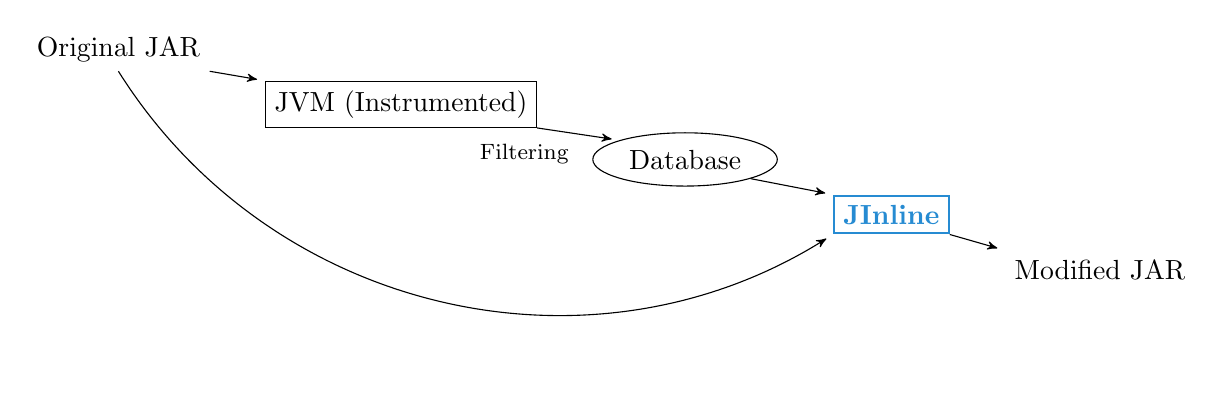
\begin{tikzpicture}[
      database/.style={ellipse, draw},
      jar/.style={},
      jvm/.style={rectangle, draw},
      ours/.style={rectangle, draw, blue, thick},
      node distance=0.7cm, ->, >=stealth', shorten >=1mm
    ]
      \node [jar] (original) {Original JAR};
      \node [jvm, right=of original, yshift=-0.7cm] (jvm) {JVM (Instrumented)};
      \node [database, right=of jvm, yshift=-0.7cm] (database) {Database};
      \node [ours, right=of database, yshift=-0.7cm] (jinliner)
            {\bfseries JInline};
      \node [jar, right=of jinliner, yshift=-0.7cm] (modified) {Modified JAR};

      \path (original.south east) edge (jvm.north west)
            (jvm.south east) edge
              node [below left] {\footnotesize Filtering} (database.north west)
            (database.south east) edge (jinliner.north west)
            (original.south) edge [bend right=45] (jinliner.south west)
            (jinliner.south east) edge (modified.north west);
    \end{tikzpicture}
  \end{frame}

  \begin{frame}[fragile]
    \frametitle{We Extract Inline Targets from the JVM}

    \begin{lstlisting}[xleftmargin=9em]
public class Application {
  // ...
  public void bar() {
    o.foo();
  }
  // ...
}
    \end{lstlisting}

    \vspace{1em}
    An inline target consists of a \structure{callsite} and \structure{callee}:
    ~\texttt{\small Application.bar@0 C.foo}
  \end{frame}

  \begin{frame}[fragile]
    \frametitle{Our Database Contains the Safe Inlinings}

    \begin{tikzpicture}[remember picture, overlay, ->, >=stealth', shorten >=2mm, blue]
      \draw ($(pic cs:line-bci-4-end)+(6em,0.4em)$)
        node [right] {Safe to inline}
        --
        ($(pic cs:line-bci-4-end)+(0,0.4em)$);
      \draw ($(pic cs:line-bci-7-end)+(6em,0.4em)$)
        node [right] {Unsafe to inline}
        --
        ($(pic cs:line-bci-7-end)+(0,0.4em)$);
    \end{tikzpicture}
        \begin{lstlisting}[xleftmargin=9em, name=bci]
public class Application {
  // ...
  public void bar() {
    o.foo(); /* resolves to
                C.foo */
    // ...
    o.foo(); /* resolves to
                many different
                .foo methods */
  }
  // ...
}
        \end{lstlisting}
  \end{frame}

  \begin{frame}
    \frametitle{JInline Leverages Soot to Transform JARs}

    \structure{Soot:} framework for analyzing and transforming Java applications

    \vspace{2em}
    Our implementation:
    \begin{itemize}
      \item Modified Soot to track bytecode indices
      \item Reads safe inlining targets from the database
      \item Uses Soot to statically inline
    \end{itemize}
  \end{frame}

  \begin{frame}
    \frametitle{3 Major Factors Apply to Unsafe Inline Targets}

    The major factors are:
    \begin{itemize}
      \item Size restrictions (program size explosion)
      \item Recursion (both direct and indirect)
      \item Virtual call has multiple targets
    \end{itemize}
  \end{frame}

  \begin{frame}[fragile]
    \frametitle{We Extended JInline to Handle Multi-Typed Callsites}

    If a callsite only has one type at runtime, just inline that type

    \vspace{2em}

    We extend this idea to multiple types

    \vspace{4em}

    \texttt{o.foo} becomes:
    \begin{lstlisting}
if type(o) == A:
    /* inlined body of A.foo */
else if type(o) == B:
    /* inlined body of B.foo */
    \end{lstlisting}
  \end{frame}

  \begin{frame}
    \frametitle{JInline Maintains a Reasonable Program Size}

    \centering
    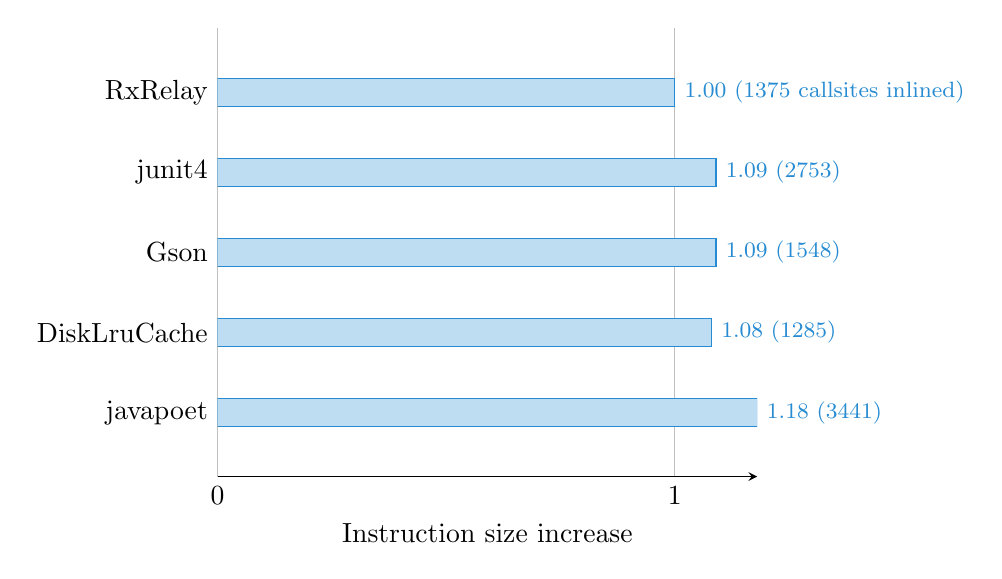
\begin{tikzpicture}
      \begin{axis}[
        xbar,
        xmin = 0,
        xtick={0,1},
        xticklabels={0,1},
        axis x line = bottom,
        xlabel = {Instruction size increase},
        xmajorgrids,
        axis y line = left,
        y axis line style = { draw=none },
        enlarge y limits  = 0.2,
        tickwidth=0pt,
        symbolic y coords = {javapoet, DiskLruCache, Gson, junit4, RxRelay},
        nodes near coords,
        nodes near coords style={font=\footnotesize},
        nodes near coords align={anchor=west},
        point meta=explicit symbolic,
      ]
        \addplot coordinates {
          (1.18,javapoet) [1.18 (3441)]
          (1.08,DiskLruCache) [1.08 (1285)]
          (1.09,Gson) [1.09 (1548)]
          (1.09,junit4) [1.09 (2753)]
          (1,RxRelay) [1.00 (1375 callsites inlined)]
        };
      \end{axis}
    \end{tikzpicture}
  \end{frame}

  \begin{frame}
    \frametitle{Future JInline Work}

    Currently, JInline aggressively inlines everything that it can

    \vspace{2em}

    Instead, we can inline a method only when it helps the other tools
  \end{frame}

  \begin{frame}
    \frametitle{We Can Improve Inlining at Runtime}

    Currently we use the JVM's decisions as the ``ground truth'' for our inline
    targets

    \vspace{2em}

    We looked more closely into how the JVM makes inlining decisions
  \end{frame}

  \begin{frame}
    \frametitle{Current Work: Improving JIT Inlining}
    The JVM's current profiling for inline targets is very simple

    \hspace{1em} Fixed heuristics

    \vspace{2em}

    Goal: learn better inlining decisions using machine learning
  \end{frame}

\end{document}
